
\chapter{Solar wind and CME influence on the magnetosphere}
\label{chap:chapter2}

Impact estimations derived from empirical correlations between in-situ solar-wind measurements and the geomagnetic \Kp{}~index\\

%\section{Abstract}

%context
Variations in the Earth's magnetosphere are largely evoked by influence through the solar wind. These magnetospheric disturbances have diverse effects on the terrestrial environment. Especially the effects of severe geomagnetic storms created by coronal mass ejections (CMEs) pose various threats to sensitive technical systems and exposed humans. Thus, the development of quantitative forecasts for magnetospheric impacts caused by solar wind and CMEs is of major importance. The analyses in this chapter are based on my work done for the project Advanced Forecast For Ensuring Communications Through Space (AFFECTS).

%aims
This study's goals are to estimate the magnetospheric impact from solar activity in general, from solar wind and also to predict it for CMEs in particular. Empirical dependencies between specific solar-wind parameters and the magnetospheric disturbance index~\Kp{} are presented. These dependencies allow to nowcast the \Kp~index from upstream (L1) solar-wind in-situ measurements. Hence, also the magnetospheric impact of CMEs is estimated solely based on their arrival velocities, predicted from coronagraph observations. The prediction of solar-wind stream velocities, e.g., from coronal hole observations, enables to estimate their impact as well.

%methods
First, I estimate the long-term variations of the yearly average \Kp{}~values, which are contributed by solar activity. This is achieved via logarithmic fitting of a yearly sunspot number (SSN) dependency. In order to nowcast the \Kp~index from general solar-wind conditions, I apply a correlation with the product of the parameters velocity and magnetic field z\~component in GSM coordinates (\vBz{}). In order to forecast the \Kp~index from estimated CME and stream velocities, I furthermore filter the solar-wind data, using flagged CME times from the solar-wind structures (SWS) list provided by \citet{Richardson2012}. The solar-wind data considered in these analyses consists of 35~years (1981--2016) of high-resolution minutely OMNI data, which is composed of multi-spacecraft intercalibrated in-situ measurements from \SI{1}{\au}. I evaluate various data processing methods and choose the methods resulting in the highest correlation coefficients with \Kp{}. I analyze the \Kp{} frequency distributions with respect to the depending parameters \vBz{} and velocity, derive their mean \Kp{} per interval and further compile functional dependencies via logarithmic fitting.

%results
The obtained functional relations enable to empirically estimate the mean \Kp{} impact from measured solar activity, in-situ solar wind, and remotely determined CME and stream velocities.

%conclusions


\section{Introduction}
%%% motivation
It is known since the early 19th~century that variations in the solar wind evoke disturbances in the magnetosphere \citep{Bartels1962}. Especially strong disturbances, called geomagnetic storms, can be provoked by coronal mass ejections (CMEs), which are embedded within the solar wind. The causes of the strongest geomagnetic storms are the compression of the solar-wind magnetic field lines within the CME shock front and the enhanced field strenghts of magnetic clouds, which are enclosed in CMEs \citep{Bothmer1993}. The consequences of strong geomagnetic disturbances are a threat to sensitive technical systems and exposed humans. Therefore it is important to know when magnetospheric disturbances will occur and how large they will become.\\

\Kp{} is designed for... (cite?). I use this magnetospheric disturbance index to correlate it with near-Earth solar-wind measurements. More detailed information on the \Kp{}~index can be found in \autoref{sec:kp_index}.\\

current comparable \Kp~forecast models take into account...\\
\citet{Elliott2013}: The \Kp~index and solar-wind speed relationship: Insights for improving space weather forecasts\\
differences to existing studies:\\
here I show...\\

%results
With the results presented in this chapter, I elaborate the step from the predicted CME and stream velocities to the forecast of the possible impact strength on the terrestrial magnetosphere. I derive an empirical correlation between the solar-wind speed and the geomagnetic \Kp~index, in order to obtain the capability to forecast \Kp{} values solely based on the predicted CME and stream velocities. The derived functional dependencies can be used to nowcast/forecast the \Kp~index.\\

%general solar-wind nowcast; rt-data
In-situ measurements of solar wind are made almost continuously, e.g., at the first Lagrange point (L1), in front of the magnetosphere. Since 1963 several spacecraft collected more than 50~years of data. The latest spacecraft, e.g., Wind, ACE and DSCOVR (launched in early 2015), provide real-time solar-wind data online\footnote{Wind real-time data website: \url{https://pwg.gsfc.nasa.gov/windnrt/}} \footnote{ACE real-time data website: \url{http://www.swpc.noaa.gov/products/ace-real-time-solar-wind}} \footnote{DSCOVR real-time data website: \url{http://www.swpc.noaa.gov/products/real-time-solar-wind}}.
% solar wind impacts
These solar-wind real-time data are used to nowcast various effects on the Earth's magnetosphere, such as the position of the magnetospheric bow shock in front of the Earth, the magnitude of geomagnetic disturbances (e.g., \Kp~index), the positions of the polar auroral ovals, the variation of the total electron content (TEC) of the ionosphere, and the positional error of global navigation satellite systems (GNSS).\\


%CME velocity forecast
The velocity and the direction of CMEs can be determined in their early near-Sun stages via remote tracking with coronagraph white-light observations. Using these parameters as input for CME propagation models, their possible arrival time and arrival velocity at Earth can be derived.\\

%stream velocity forecast from CHs
Coronal holes are the origin of the fast solar wind; their area on the solar disk, seen in EUV wavelengths, correlates with the measured velocity of solar-wind streams \citep{Vrsnak2007}. This relation is used to predict the Earth-arrival velocity of solar-wind streams about 4~days in advance \citep{Rotter2012}, as is done in real-time within the empirical solar-wind forecast (ESWF) at the University of Graz\footnote{ESWF website: \url{http://swe.uni-graz.at/index.php/services/solar-wind-forecast}}.\\

%%% synopsis
For the analyses performed and found in this chapter, the objectives are to estimate the magnetospheric impact of solar wind and to predict it for CMEs in particular. In Sect.~\ref{sec:long_term_variations} I determine the magnitudes of the long-term \Kp{} changes due to solar activity and measure the extent of seasonal variations stemming from the Earth's orbit. In order to nowcast the \Kp{}~index, I quantify the solar-wind influence on \Kp{} by deriving a functional relation with the product of solar-wind velocity and magnetic field z-component (Sect.~\ref{sec:kp_nowcast}). Finally, for the purpose of enabling \Kp{} forecasts from remote observations, I estimate the \Kp{} impact coming from CMEs and solar-wind streamers separately by deriving functional dependencies with their velocities (Sect.~\ref{sec:kp_forecast}).


\section{Long-term variations of the \Kp{}~index}
\label{sec:long_term_variations}

\subsection{Solar activity influence on the \Kp{}~index}
The \Kp{} data is obtained from the GFZ~Potsdam\footnote{GFZ~Potsdam website: \url{http://www.gfz-potsdam.de/de/kp-index/}}, where the index is currently maintained. The data used in this analysis covers the time period 1932--2016. Its frequency distribution shows that the highest frequencies occur around low \Kp{} values of 1+. Going to higher \Kp{} values, the frequencies seem to decline asymtotically towards zero (see Fig.~\ref{fig:Kp_histogram_b}) -- a \Kp{} value of 9o occurred only 29 times in this time interval.\\
\begin{figure}[htb]
	\begin{floatrow}
		\ffigbox{
			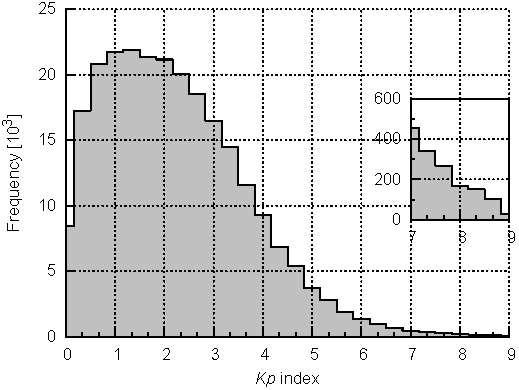
\includegraphics[width=0.5\Xhsize]{figures_of_mine/chapter2/Kp_histogram_b.pdf}
		}{
			\caption{\Kp{} frequency distribution for the time period 1932--2016. The inset shows a zoomed-in view of the high-value tail. The \Kp{} data is obtained from the GFZ~Potsdam.}
			\label{fig:Kp_histogram_b}
		}
		\ffigbox{
			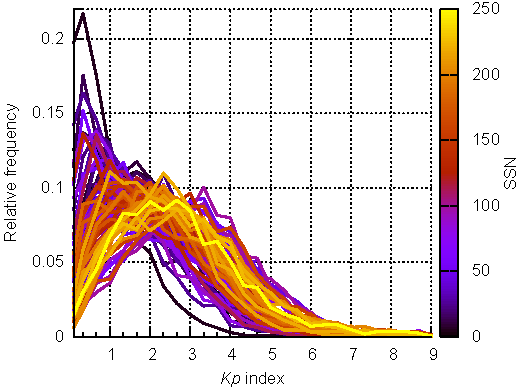
\includegraphics[width=\Xhsize]{figures_of_mine/chapter2/Kp_histogram_yearlySSN.pdf}
		}{
			\caption{Yearly \Kp{} frequency distributions during the period 1932--2016, sorted and colored by yearly SSN. All distributions are normed to be of equal area. The \Kp{} data is obtained from the GFZ~Potsdam and the yearly SSN data from the SILSO World Data Center.}
			\label{fig:Kp_histogram_yearlySSN}
		}
	\end{floatrow}
\end{figure}

Obviously the general \Kp{} distribution (seen in Fig.~\ref{fig:Kp_histogram_b}) averages over solar activity. Solar activity is generally tracked with the international sunspot number (SSN). In the present analyses its data from the time period \citeyear{sidc1917} is used. The data is obtained from the online catalog\footnote{WDC-SIDC website: \url{http://www.sidc.be/silso/}} provided by the World Data Center -- Sunspot Index and Long-term Solar Observations (WDC-SILSO), Solar Influences Data Analysis Center (SIDC), Royal Observatory of Belgium (ROB).

The \Kp{} frequency distributions' shape varies with different states of solar activity. This is visible in the yearly distributions, sorted and colored by yearly SSN in Fig.~\ref{fig:Kp_histogram_yearlySSN}.

The distribution's peak position scales with SSN, that is, a high yearly SSN results in a higher abundance of large \Kp{} values as well.

The time series of yearly average \Kp{} values of the years 1932--2016 shows an imprint of the solar cycles (see the top graphs in Fig.~\ref{fig:yearly_kp-ssn_correlation_c}).
\begin{figure}
	\fcapside[\FBwidth]{
		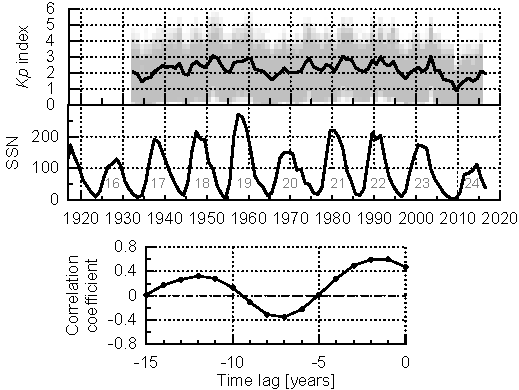
\includegraphics[width=0.6\textwidth]{figures_of_mine/chapter2/yearly_kp-ssn_correlation_c.pdf}
	}{
		\caption{Yearly \Kp~index distributions (shaded area) with their mean values for the time period 1932--2016 and yearly SSN with cycle number for the time period 1917--2016 (top panels). The Pearson correlation coefficients with the yearly SSN are calculated for time lags back to -15~years (bottom panel). The \Kp{} data is obtained from the GFZ~Potsdam and the yearly SSN data from the SILSO World Data Center.}
		\label{fig:yearly_kp-ssn_correlation_c}
	}
\end{figure}
The \Kp{} pattern follows the solar cycle minima and maxima as well as the changes in magnitude between solar cycles. The yearly mean \Kp{} shifts about 1~unit for both variations separately. As expected, the \Kp{}~index correlation with solar activity shows an 11-year period (see bottom graph in Fig.~\ref{fig:yearly_kp-ssn_correlation_c}). The highest correlation coefficient of 0.60 is found with a time lag of $-1$~year, that is, the yearly average \Kp{} follows the SSN of the previous year.
%Kp-ssn cc: 0.5971

The yearly mean \Kp~index with respect to the 1-year lagged SSN shows a raise with increasing SSN, this is seen in Fig.~\ref{fig:Kp_SSN_fit_d}.
\begin{figure}
	\fcapside[\FBwidth]{
		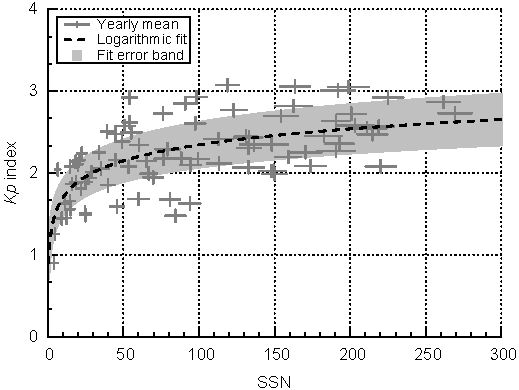
\includegraphics[width=0.6\textwidth]{figures_of_mine/chapter2/Kp_SSN_fit_d.pdf}
	}{
		\caption{Yearly mean \Kp~index with respect to 1-year lagged SSN (+) with the weighted logarithmic fit (dashed). The error bars denote the SSN standard deviation and the relative weight from the yearly data coverage. The shaded area represents the fit error band derived from the estimated standard deviations of the fit parameters. The logarithmic function, equation (\ref{eq:log_fit_function}), is used for the weighted fit. The yearly \Kp{} mean values are calculated from GFZ~Potsdam data and the yearly SSN is obtained from the SILSO World Data Center.}
		\label{fig:Kp_SSN_fit_d}
	}
\end{figure}
I perform a fit in order to obtain an analytical relation for this dependency. \Kp{} itself is a quasi-logarithmic index, so it is apparent to use a logarithmic fit function:
\begin{align}
	f(x) = a \cdot \ln(x) + b	\,.	\label{eq:log_fit_function}
\end{align}
The fit parameters are $a = 0.281(43)$ and $b = 1.05(19)$ and lead to the relation
\begin{align}
	\Kp(ssn) = 0.28 \cdot \ln(ssn) + 1.1	\,,	\label{eq:kp_ssn_relation}
\end{align}
% log fit parameters:
% a 0.281126         +/- 0.04267
% b 1.04923          +/- 0.19
which is plotted in Fig.~\ref{fig:Kp_SSN_fit_d}. This means that for a SSN of $1$ the mean \Kp{} is about $1.1$ and for a SSN of 200 it is about $2.5$. The fit error band has a width of about half a \Kp~unit.

\subsection{Seasonal variations of the \Kp{}~index}
On top of the yearly variations, seasonal variations exist in the magnetospheric disturbances as well. In the months May--August the \Kp{} peak frequency is higher than in the remaining months of the year, whereas in March/April and September/October the \Kp{} values \num{>3} are more abundant. This is apparent from looking at the monthly \Kp{} frequency distributions, plotted in Fig.~\ref{fig:Kp_histogram_monthly}.
\begin{figure}[htb]
	\begin{floatrow}
		\ffigbox{
			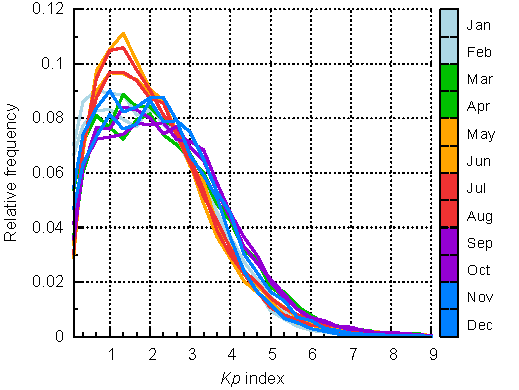
\includegraphics[width=0.5\Xhsize]{figures_of_mine/chapter2/Kp_histogram_monthly.pdf}
		}{
			\caption{Average monthly \Kp{} frequency distributions of the time period 1932--2016, colored by month of the year. The \Kp{} data is obtained from the GFZ~Potsdam.}
			\label{fig:Kp_histogram_monthly}
		}
		\ffigbox{
			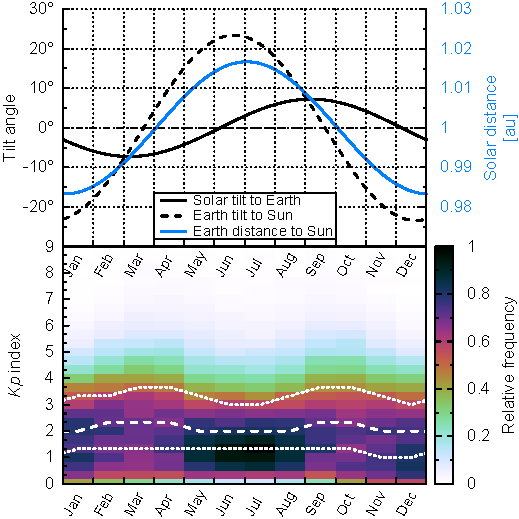
\includegraphics[width=\Xhsize]{figures_of_mine/chapter2/Kp_seasonal_c.pdf}
		}{
			\caption{Seasonal changes in the solar tilt angle to Earth, Earth tilt angle to Sun, and Earth distance to Sun -- the curves are approximated with trigonometric fuctions (top). \Kp{} frequency distributions by month for the time period 1932--2016 with median and quartile values (bottom). The bin size is 1~month and \SI{1/3}{\Kp}~unit respectively.}
			\label{fig:Kp_seasonal_c}
		}
	\end{floatrow}
\end{figure}
These \Kp{} changes arise from seasonal variations of the solar-wind parameters at Earth, which stem from Earth's yearly changes in orbital distance and heliographic latitude. Another seasonal effect stems from the Earth's rotation axis tilt, which changes the direction of the Earth's magnetic dipole axis to the Sun over the year (see top panel of Fig.~\ref{fig:Kp_seasonal_c}).

Earth's distance to the Sun varies over the course of a year by \SI{+-1.67}{\percent} (see appendix \autoref{sec:earth_orbit_geometry}). The solar-wind parameters scale via power-law dependencies with solar distance, as is described in the following \autoref{chap:empirical_solar_wind_model_for_the_inner_heliosphere} and accordingly in \citet{Venzmer2017}. For example, if the solar-wind proton density scales with $r^{-2}$, this leads to yearly variations in density of up to \SI{3.4}{\percent}. These yearly solar-wind changes have a direct influence on the \Kp{}~index.

The Sun's rotation axis tilt angle to the ecliptic is \SI{+-7.25}{\degree} and that for Earth is \SI{+-23.44}{\degree} (cite 'NASA Earth fact sheet' or U.S. Nautical Almanac Office 2015), see also appendix \autoref{sec:earth_orbit_geometry}. The solar-wind magnetic field strength varies with heliographic latitude (cite?). Furthermore, the rate of magnetic reconnection between solar wind and the Earth's magnetosphere depends on both fields' orientation to each other (parallel/antiparallel) (see also Basics, Figure XX). The solar-wind influence on the \Kp{}~index depends on its coupling efficiency with the magnetosphere. Additionally, the tilt of the magnetic dipol axis to the rotation axis -- a few degrees for the Sun during cycle minima and about \SI{10}{\degree} for the Earth -- complicates this system even more.
%geomagnetic dipole tilt: Planetary fact sheet: 11.2 (Model GSFC-12/83)
%variation range in the time period 1930--2016: 9.6--11.5° (http://wdc.kugi.kyoto-u.ac.jp/poles/polesexp.html)

So the \Kp{} variation effects originate from the seasonal changing of the solar tilt, the Earth's tilt, and the Earth's distance. A thorough analysis of these seasonal variations would require a dedicated study going beyond the scope of this work, but already was performed by XXX (cites?). Thus, I just quantify the bulk magnitude of these effects (and include them as relative uncertainties). Looking at the \Kp{} frequency distributions by month -- seen in the bottom panel of Fig.~\ref{fig:Kp_seasonal_c} -- it is apparent that for high \Kp{} values ($>4$), there exist yearly frequency maxima at the equinoxes and frequency minima at the solstices. Their variation amounts to about 1~\Kp~unit.

The changes from the \Kp{}-SSN relation (\ref{eq:kp_ssn_relation}) and the seasonal variations are of similar order (about 1~\Kp{}~unit).\\


causes (see citet{Rangarajan1997} p.~1282 and mention Bartels1963 too)\\
read Bothmer1998 Ch 3...\\


into thesis:\\
NASA maintains the Planetary~Fact~Sheets\footnote{NASA Planetary Fact Sheets website: \url{https://nssdc.gsfc.nasa.gov/planetary/planetfact.html}} online, which are quite useful.\\


\section{Solar wind-magnetosphere coupling}
%literature
The coupling between the solar wind and the magnetosphere is governed by reconnection and compression of the magnetic field lines (see Basics...).\\

the dayside reconnection is asymmetric\\
half-wave rectifier coupling\\
To describe this, coupling functions with different complexity were proposed (Newell, cites? and list).\\

In this work I settle for \vBz{} as the coupling function.\\

It makes sense to use the geocentric solar magnetospheric (GSM) coordinate system, which is aligned with the Earth's magnetic dipole axis.\\

dayside reconnection:\\
``$E_\text{y}$ is the rate at which southward magnetic flux is convected to the magnetosphere by the solar wind ($-v_\text{x} \cdot B_\text{z}$) in GSM coordinates,'' \citep{Russell2007}\\

The solar wind electric field $E_y$ is the product of the proton velocity $v$ and the magnetic field z-component $B_\text{z}$:
\begin{align}
	?check vectors  E_\text{y} = -v_\text{x} \times B_\text{z}\,.	\label{eq:coupling_vxB}
\end{align}
If not specified otherwise, $B_\text{z}$ is always meant to be in GSM coordinates hereafter.\\

The solar wind velocity sticks mostly to its radial flow direction, that is, it only rarely deviates up to \SI{0.0}{\degree} (correct and cite...). Thus, the absolute flow speed can be used instead of the vector component.\\

argue for \vBz:\\
- 3hmin(\vBz) performs in rank correlation slightly better than the sophisticated Newell formula. really?\\
- simple to calculate\\
- ...\\

It is also known that the solar-wind velocity itself already correlates strongly with the \Kp~index. In fact, \citet{Machol2013} even proposed a linear function of the \Kp~index as a best proxy for corrupted real-time velocity measurements made by the Advanced Composition Explorer (ACE) spacecraft.\\

I use this velocity relationship for obtaining \Kp{} proxies from CME and solar wind stream data.\\


\section{\Kp{} nowcast from in-situ solar-wind measurements}
\label{sec:kp_nowcast}

\subsection{Data set, data processing and correlation}
\label{sec:data_set__data_processing_and_correlation}
%determine data basis
The \Kp{} time series started in 1932 when there existed no spacecraft to measure solar wind in~situ. Thus, the surveyed time range is defined by the available in-situ solar-wind data.\\

%argue for averaging method
The \Kp{}~index represents maximal variations within 3-hour time intervals (see \autoref{sec:kp_index}). Any solar-wind parameter that will be correlated with \Kp{} also has to have the same time resolution. In addition to adapting the time resolution, it has to be considered by which means this should be done. Simple 3-hour average values are expected to have a lower correlation coefficient than the solar-wind parameter's 3-hourly maximal variation.
%argue for high resolution, deliberate between hourly and minutely data
The 3-hour maximal variations are obviously higher when using high resolution data. Thus, to be able to correlate \Kp{} with solar-wind data, high resolution data (e.g., 1~min) is needed to determine the maximal solar-wind variations within each 3-hour interval.\\

The OMNI data set collects the longest continuous solar-wind measurements at \SI{1}{\au}. The longest time coverage has the hourly OMNI data set (since 1963), however, I prefer to use the minutely OMNI data with the time range 1981--2016. [to benefit from higer correlation coefficients (see Figs?).]\\

why this data set? - because of long time coverage, to magnetospheric bow shock calculated solar wind and integrated geomagnetic indices (see Paper...)\\

The \Kp{}-\vBz{} Pearson correlation coefficients for 3-hour mean and minimum data are plotted in Fig.~\ref{fig:cc_lag_data_d_KpvsVBzgsm}.
\begin{figure}[htb]
	\begin{floatrow}
		\ffigbox{
			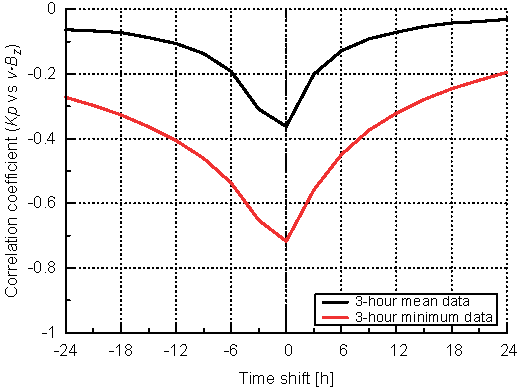
\includegraphics[width=0.5\Xhsize]{figures_of_mine/chapter2/cc_lag_data_d_KpvsVBzgsm.pdf}
		}{
			\caption{\Kp-\vBz{} correlation coefficients for different time shifts up to \num{+-24}~hours. Minutely OMNI data from 1981--2016 processed with mean (black) and minimum (red) 3-hour averaging.}
			\label{fig:cc_lag_data_d_KpvsVBzgsm}
		}
%highest correlation coefficients:
%min:	0.00000    -0.717240
%mean:	0.00000    -0.362237
%max:	0.00000     0.293137
		\ffigbox{
			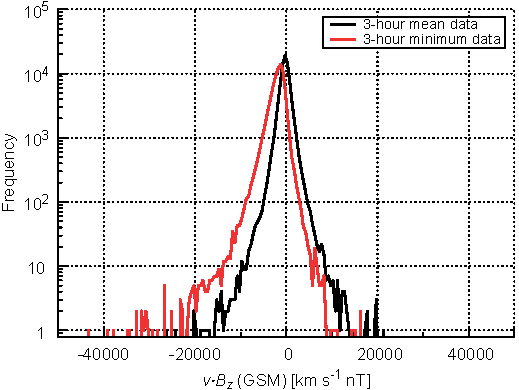
\includegraphics[width=\Xhsize]{figures_of_mine/chapter2/histogram_VBzgsm.pdf}
		}{
			\caption{Frequency distributions of \vBz{} for 3-hour mean (black) and minimum (red) minutely OMNI data from 1981--2016.}
			\label{fig:histogram_VBzgsm}
		}
%vBz frequency shifts:
% min shift: -1250
% mean shift: -250
% max shift: -750
	\end{floatrow}
\end{figure}
The largest correlation is found for the 3-hour minimum data without time shift. It is a negative correlation with a coefficient of $-0.72$. For \vBz{} 3-hour minimum values, their frequency distribution and its peak is asymmetrically shifted to negative values, as seen in Fig.~\ref{fig:histogram_VBzgsm}.


\subsection{Functional dependency for solar wind}
%distribution
The frequency distribution in \Kp-\vBz{} space is shaped like a candle flame, inclined to negative values by a light breeze, see top panel in Fig.~\ref{fig:Kp_2dhistogram_VBzgsm_sws_e}.
\begin{figure}
	\fcapside[\FBwidth]{
		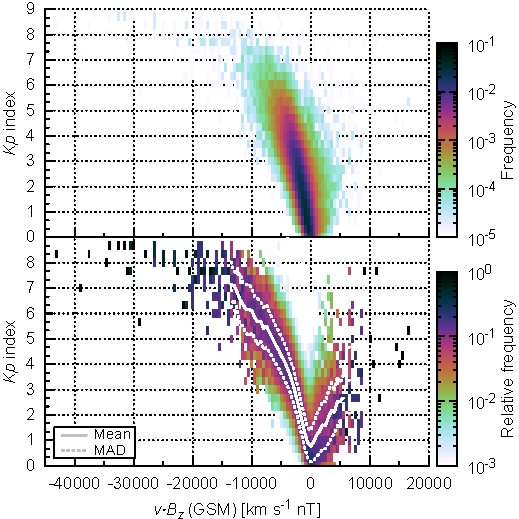
\includegraphics[width=0.6\textwidth]{figures_of_mine/chapter2/Kp_2dhistogram_VBzgsm_sws_e.pdf}
	}{
		\caption{\Kp{} versus \vBz{} frequency distribution (top) and its relative distribution (bottom) with the mean \Kp{} values (solid) and their mean absolute deviation (dotted). It is 3-hour minimum data from the minutely OMNI data set (1981--2016). The bin size is \SI{500}{\km\per\s\nano\tesla} and \SI{1/3}{\Kp}~unit respectively.}
		\label{fig:Kp_2dhistogram_VBzgsm_sws_e}
	}
\end{figure}
%dependency
In order to determine a functional dependency, I focus on the relative frequencies per \vBz-interval and their mean \Kp{} values, which are plotted in the bottom panel of Fig.~\ref{fig:Kp_2dhistogram_VBzgsm_sws_e}. The mean absolute deviation (MAD) of the mean has a mean size of \SI{0.7}{\Kp}~units. This probability distribution is asymmetrically V-shaped around zero, having a larger and steeper negative arm than positive arm. The asymmetry also exists for 3-hour mean data, thus this effect is not a result of the data reducing method (3-hour minimum) (fig...?). Rather the steeper negative arm is a consequence of the half-wave rectifier coupling of the solar-wind magnetic field direction to the magnetosphere, as described in \autoref{sec:solar_wind_magnetosphere_coupling}.\\
%MAD: 2.211/3 = 0.737 Kp units

%determine fitting functions
Since the \Kp~index has a quasi-logarithmic scaling (see \autoref{sec:kp_index}), a logarithmic function is the obvious choice as a fit function. Furthermore, the depending argument consists of a product of two solar-wind parameters which individually scale logarithmically with \Kp{}. These reasons are why I use the logarithm of a parabola for the fitting approach:
\begin{align}
	f(x) &= \ln\left(x^2\right)	\,.	\label{eq:log_square_function}
\end{align}
I also introduce a horizontal shifting parameter $x'$ because the distribution's center is slightly offset. To be able to replicate the asymmetry in both arms, I further split the fit function into a negative and a positive part:
\begin{align}
	f(x) &=
	\begin{cases}
		\,f_-(x) &\text{for } x < 0	\,,\\
		\,f_+(x) &\text{for } x \ge 0	\,.
	\end{cases}	\label{eq:log_square_fit_function}
\end{align}
This way, both arms can be scaled individually with the scaling factors for the negative and positive parts $a_-$ and $a_+$. The resulting logarithmic fit functions are
\begin{align}
	f_-(x) &= a_- \cdot \ln\left(\left(x + x'\right)^2 + b\right) + y'	\,,\\
	f_+(x) &= a_+ \cdot \left(f_-(x) - f_-\left(-x'\right)\right) + f_-\left(-x'\right)	\,,
\end{align}
with the vertical shifting parameter $y'$ and the depth parameter $b$. The resulting fit curve is plotted in Fig.~\ref{fig:Kp_2dhistogram_VBzgsm_sws_fit_e} with the fit coefficients $a_- = 1.258(19)$, $y' = -17.04(33)$, $a_+ = 0.467(20)$, $b = \num{1.416(68)e6}$, and $x' = 163(20)$ for units of [\si{\km\per\s \nano\tesla}].
%high precision values:
% a_- = 1.25788(0.019)\\
% y' = -17.0394(0.33)\\
% a_+ = 0.467039(0.0197)\\
% b = 1.41639e6(0.067795e6)\\
% x' = 162.907(20.642)\\
\begin{figure}
	\fcapside[\FBwidth]{
		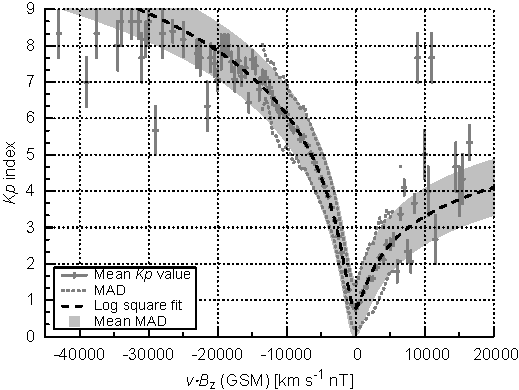
\includegraphics[width=0.6\textwidth]{figures_of_mine/chapter2/Kp_2dhistogram_VBzgsm_sws_fit_e.pdf}
	}{
		\caption{Mean \Kp{} values (+) and MAD values (dotted) per \vBz~interval. The error bars represent the relative data count. The logarithmic fit (dashed) is plotted with a mean MAD band (shaded area). The splitted function (\ref{eq:log_square_fit_function}) is used for the weighted fit.}
		\label{fig:Kp_2dhistogram_VBzgsm_sws_fit_e}
	}
\end{figure}
The mean MAD is about 0.7~\Kp{}~units. Thus, the solar-wind dependency relation condenses to:
\begin{align}
	\text{\Kp}_-\left(vB_\text{z}\right) &= 1.258 \cdot \ln\left(\left(vB_\text{z} + 163\right)^2 + \num{1.416e6}\right) - 17.04	\,,	\label{eq:kpvsvbz_dependency_function_negative}\\
	\text{\Kp}_+\left(vB_\text{z}\right) &= 0.467 \cdot \left(\text{\Kp}_-\left(vB_\text{z}\right) - \text{\Kp}_-(-163)\right) + \text{\Kp}_-(-163)	\,.	\label{eq:kpvsvbz_dependency_function_positive}
\end{align}
This relation can be used together with real-time in-situ measurements from spacecraft located at L1 (see Section~XX rt sources) to nowcast the actual \Kp~index.


\section{\Kp{} forecast from remote CME and stream observations}
\label{sec:kp_forecast}
%CMEs
CMEs are already sighted raising from their source regions on the solar surface. Some CME properties can be estimated from remote coronagraph observations and modeled to Earth, such as its propagation direction, its arrival time, and arrival velocity (cites?). Thus, early observations enable a heads-up time only depending on the CME's propagation speed to Earth. This travel duration can be more than 4~days for slow events with average solar-wind speeds, about 40~hours for fast events with speeds of \SI{1000}{\km\per\s}, and down to 20~hours and even below for the rare extreme cases, e.g., about 21~hours for the event on 23~July 2012 \citep{Russell2013,Temmer2015} and about 19~hours for the event observed by \citet{Carrington1859} on 1~September 1859.

To make use of the heads-up time for CMEs, I neglect its magnetic field part, which can hardly be determined from remote observations and simplify the coupling relation (\ref{eq:coupling_vxB}) from before. Therefore, the only coupling parameter remaining is the solar-wind velocity.

\subsection{CME velocity estimation}
methods and modeling...?\\
GCS, CAD modeling -> propagation direction and apex height-time profile -> acceleration and velocity kinematics...\\
-> example event CME?\\

\subsection{Solar wind stream velocity estimation}
CH analysis (Graz)\\
L4 shift (Graz)\\
WSA-ENLIL MHD simulation\\

\subsection{SWS CME list}
For the following analysis, I use the list of solar-wind structures (SWS) created and updated by \citet{Richardson2000} and \citet{Richardson2012}, who characterized the near-Earth solar-wind structures since 1963. All periods related to ICMEs in the OMNI solar-wind data set were identified and flagged.\\

list identifying criteria...\\

The SWS list for 1963--2016 was kindly provided by Ian~Richardson (private communication). into acknowledgments...\\

SWS list for 1963--2015 by \citep{Richardson2000,Richardson2012} is available via registration at CEDARweb\footnote{CEDARweb website for Solar Wind Structures: \url{http://cedarweb.vsp.ucar.edu/wiki/index.php/Tools_and_Models:Solar_Wind_Structures} (existent in 2017-10-29)}.\\
List of near-Earth ICMEs since January 1996 by \citet{Cane2003,Richardson2010}. Available as ACE Level~3 data for the period 1995--mid2016\footnote{ACE Level~3 data website -- list of near-Earth ICMEs: \url{http://www.srl.caltech.edu/ACE/ASC/DATA/level3/icmetable2.htm} (existent in 2017-10-29)}.\\

The CME fraction in the OMNI data is \SI{15.8}{\%} during the time period 1981--2016 (this accumulates to 5.53~years).
%and that for the period 1963--2016 is \SI{17.0}{\%} (9.01~years).\\
This percentage is an average value. It varies heavily with the solar activity cycle and with the appearance of individual active regions on the solar surface. In the following, I refer to the remaining part without CMEs as ``solar-wind streams'', because it is composed entirely from a mixture of slow wind flows, fast wind streams, and their interaction regions.

% acknowledgments:\\
% The hourly solar-wind structure list was kindly provided by Ian~Richardson of the NASA Goddard Space Flight Center and CRESST/University of Maryland via the CEDAR Database at the National Center for Atmospheric Research, which is supported by the National Science Foundation.\\

\subsection{Data processing and correlation}
Again, I calculate 3-hour extreme values using the minutely OMNI data to profit from higher correlation coefficients, as done before for the data processing of the \vBz{} analysis in Sect.~\ref{sec:data_set__data_processing_and_correlation}. The velocity has only positive values, thus its extreme values are 3-hour maximum values. The comparison between the 3-hour maximum and the 3-hour mean frequency distributions shows that their mean position shifts from a velocity of 405 to \SI{425}{\km\per\s}, see Fig.~\ref{fig:histogram_V_b}.
%the SWS1 mean raises from 435 to 455~km/s in 3hmax data...\\
\begin{figure}[htb]
	\begin{floatrow}
		\ffigbox{
			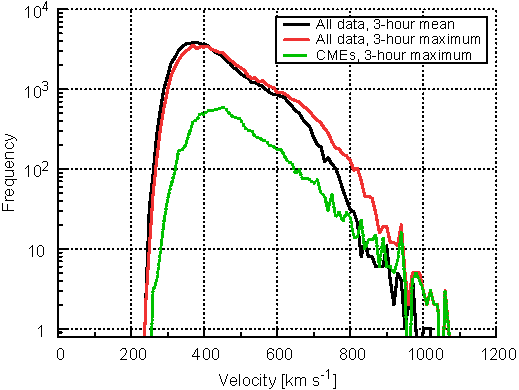
\includegraphics[width=0.5\Xhsize]{figures_of_mine/chapter2/histogram_V_b.pdf}
		}{
			\caption{Solar-wind velocity frequency distributions for 3-hour mean (black), maximum (red) and maximum of the CME part (green). Minutely OMNI data from the period 1981--2016 is used.}
			\label{fig:histogram_V_b}
		}
		\ffigbox{
			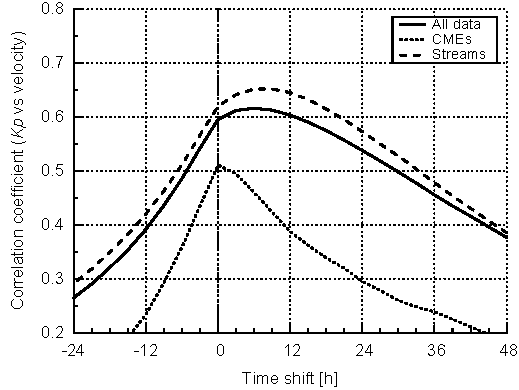
\includegraphics[width=\Xhsize]{figures_of_mine/chapter2/cc_lag_sws_d.pdf}
		}{
			\caption{\Kp{}-velocity correlation coefficients for time shifts in the range \numrange{-24}{48}~hours. The correlations for the whole solar-wind data (solid), for solar-wind streams without CMEs (dashed) and for CMEs only (dotted) are plotted. The data used is the 3-hour maximum of the minutely high resolution OMNI data from the period 1981--2016.}
			\label{fig:cc_lag_sws_d}
		}
	\end{floatrow}
\end{figure}
The CME part and solar-wind stream part of the data can be examined separately, using the CME related periods from the SWS list as a filter. Their frequency distributions show that the CME share is rising in faster solar wind until eventually in the region above about \SI{900}{\km\per\s} there only exist CMEs, see Fig.~\ref{fig:histogram_V_b}.

The CME part of the data is correlated with the \Kp~index independently from the remaining solar-wind streams, see Fig.~\ref{fig:cc_lag_sws_d}. The correlation for CME related data is lower than that for the regular solar wind (all data). Its maximal correlation coefficient with a value of 0.51 is without time shift, see Table~\ref{tab:correlation_coefficients_kpvsv}.
\begin{table*}
	\caption{Time lags with the highest correlation coefficients for the \Kp{}-velocity relation for the whole OMNI data, for stream data, and for CME data. The values are based on the 3-hour maximum of the minutely high resolution OMNI data from the time period 1981--2016.}
	\label{tab:correlation_coefficients_kpvsv}
	\centering
	\begin{tabular}{lcc}
		\hline\hline
		Data	&Time lag [hours]	&Correlation coefficient\\
		\hline
		All data	&6	&0.622\\
		Streams	&9	&0.661\\
		CMEs	&0	&0.511\\
		\hline
	\end{tabular}
\end{table*}
% the best lag times are:\\
% sws: +6 h\\
% sws1: 0 h\\
% sws23: +9 h\\
% 
% correlation coefficients\\
% SWS1\\
% 0	0.511093\\
% SWS23\\
% lag	cross	auto x	auto y\\
% -3	0.660694\\
% 0	0.620113\\
% SWS\\
% lag	cross	auto x	auto y\\
% -2	0.621539\\
% 0	0.595784\\
The solar-wind streams show a higher correlation with \Kp{} and the maximal coefficient of 0.66 has a positive time shift of 9~hours, that is, the \Kp~index forecasts the velocity of solar-wind streams 9~hours in advance.

The positive time shift can be explained with the occurence of interaction regions followed by high speed streams (HSS). When a slow solar-wind stream is followed by a fast one, the compression at their interface leads to enhanced solar-wind densities and magnetic field strengths. The peak velocity of a HSS naturally appears after the interaction region. Therefore the \Kp-impact from the enhanced magnetic field is correlated with the higher velocity of the HSS, yielding the observed positive time shift.


\subsection{Functional dependency for CME velocity}
The general \Kp-velocity dependency in the solar wind is apparent in the tilt of its distribution, see top panel of Fig.~\ref{fig:Kp_2dhistogram_V_sws_d}.
\begin{figure}
	\fcapside[\FBwidth]{
		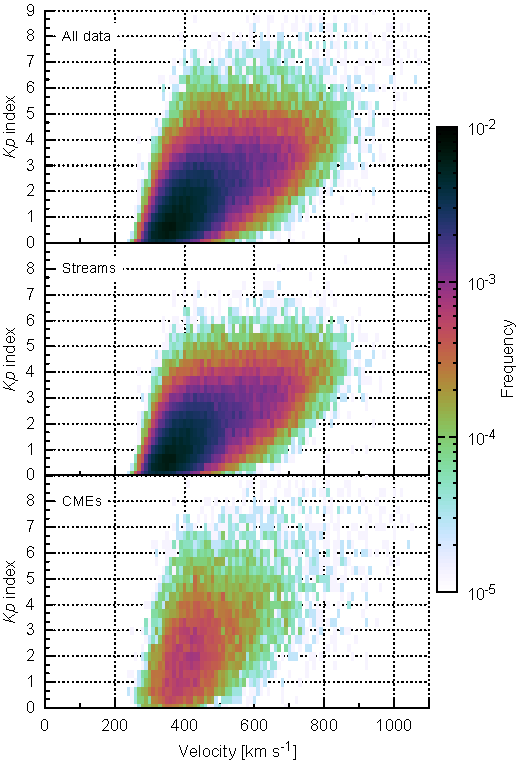
\includegraphics[width=0.6\textwidth]{figures_of_mine/chapter2/Kp_2dhistogram_V_sws_d.pdf}
	}{
		\caption{\Kp-velocity distributions for all solar-wind data, for solar-wind streams and for CMEs. The data used is the 3-hour maximum of the minutely high resolution OMNI data. The SWS list from \citet{Richardson2012} is used for the CME and stream separation. The bin size is \SI{10}{\km\per\s} and \SI{1/3}{\Kp}~unit respectively.}
		\label{fig:Kp_2dhistogram_V_sws_d}
	}
\end{figure}
The distribution is inclined to positive values and very broad. The comparison with the CME data shows that \Kp{} values \num{>6} and velocities \SI{>850}{\km\per\s} are almost always associated with CME related periods, see middle and bottom panel of Fig.~\ref{fig:Kp_2dhistogram_V_sws_d}.

To find a functional relation for the mean \Kp{} value, I look at the relative frequencies per velocity interval, which are plotted in the bottom panel of Fig.~\ref{fig:Kp_2dhistogram_V_sws1_c2}.
\begin{figure}
	\fcapside[\FBwidth]{
		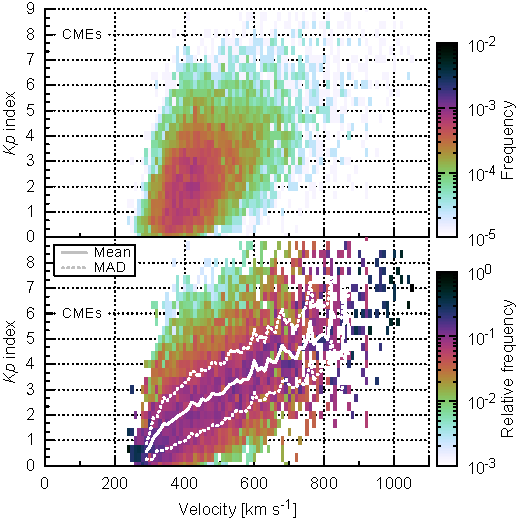
\includegraphics[width=0.6\textwidth]{figures_of_mine/chapter2/Kp_2dhistogram_V_sws1_c2.pdf}
	}{
		\caption{CME part of the \Kp-velocity distribution (same as third panel of Fig.~\ref{fig:Kp_2dhistogram_V_sws_d}) and its relative distribution per velocity interval with the mean \Kp{} values (solid) and their mean absolute deviation (dotted). The bin size is \SI{10}{\km\per\s} and \SI{1/3}{\Kp}~unit respectively. The CME part of the OMNI data from the period 1981--2016 is obtained using the SWS list from \citet{Richardson2012}.}
		\label{fig:Kp_2dhistogram_V_sws1_c2}
	}
\end{figure}
The mean \Kp{} value seems to scale almost linear with the solar-wind velocity. The MAD of the mean has a mean size of about \SI{1.1}{\Kp~units}.
%MAD: 3.338/3 = 1.113 Kp units

%determine fitting function
Again, as the \Kp~index has a quasi-logarithmic scaling, a logarithmic function is the obvious choice for the fitting process. Thus, the logarithmic function
\begin{align}
	f(x) = a \cdot \ln\left(x + x'\right) + y'	\label{eq:log_offset_fit_function}
\end{align}
is used for the fit, with the scaling factor $a$, the location parameter $x'$, and the vertical shifting parameter $y'$. The resulting fit is plotted in Fig.~\ref{fig:Kp_2dhistogram_V_sws1_fit_e} and its parameters are $a = \num{10.6(34)}$, $b = \num{-73(28)}$, and $x' = \num{8.1(43)e2}$, with the velocity in units of [\si{\km\per\s}]. The MAD is about 1.1~\Kp{} units.
%10.6075 (3.4)\\
%-73.1694 (28.)\\
%806.943 (430)\\
\begin{figure}
	\fcapside[\FBwidth]{
		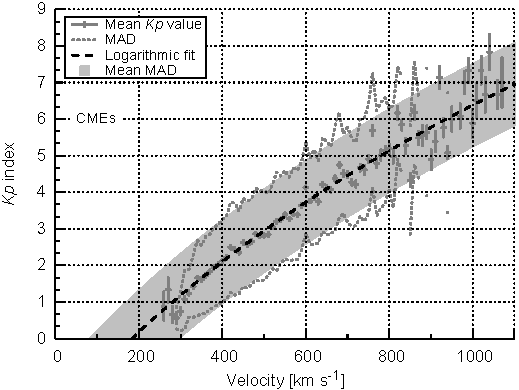
\includegraphics[width=0.6\textwidth]{figures_of_mine/chapter2/Kp_2dhistogram_V_sws1_fit_e.pdf}
	}{
		\caption{Mean \Kp{} values (+) and MAD values (dotted) per velocity interval for the CME part of the data. The error bars represent the relative data count. The logarithmic fit (dashed) is plotted with a mean MAD band (shaded area). The function (\ref{eq:log_offset_fit_function}) is used for the weighted fit.}
		\label{fig:Kp_2dhistogram_V_sws1_fit_e}
	}
\end{figure}
This leads to the CME dependency function
\begin{align}
	\Kp(v) = 10.6 \cdot \ln(v + 810) - 73	\,,	\label{eq:kpvsv_dependency_function}
\end{align}
which can be used to forecast the \Kp{}~index from the estimated CME arrival velocity.

\subsection{Functional dependency for stream velocity}
The analysis procedure in this section is similar to that in the previous section. The correlation coefficient is higher for solar-wind stream velocities when the data is shifted by 9~hours, see Fig.~\ref{fig:cc_lag_sws_d}.
I use the shifted data and look at the relative frequencies per velocity interval in order to find a functional dependency for the mean \Kp{} value, see bottom panel of Fig.~\ref{fig:Kp_2dhistogram_V_sws23_d}.
\begin{figure}
	\fcapside[\FBwidth]{
		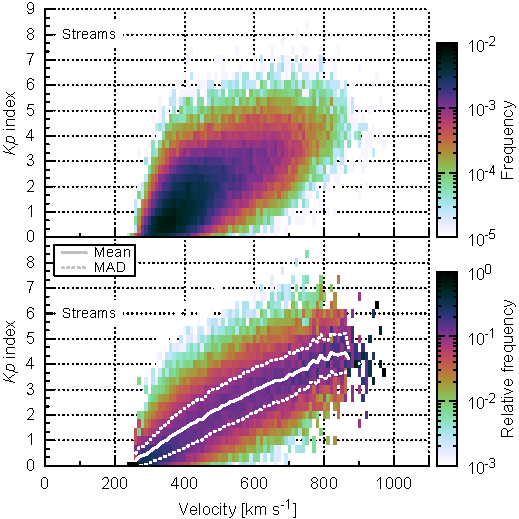
\includegraphics[width=0.6\textwidth]{figures_of_mine/chapter2/Kp_2dhistogram_V_sws23_d.pdf}
	}{
		\caption{Stream part of the \Kp-velocity distribution (similar to second panel of Fig.~\ref{fig:Kp_2dhistogram_V_sws_d}, but with the data shifted by 9-hours) and its relative distribution per velocity interval with the mean \Kp{} values (solid) and their mean absolute deviation (dotted). The bin size is \SI{10}{\km\per\s} and \SI{1/3}{\Kp}~unit respectively. The stream part of the OMNI data from the period 1981--2016 is obtained using the SWS list from \citet{Richardson2012}.}
		\label{fig:Kp_2dhistogram_V_sws23_d}
	}
\end{figure}
Again, the mean \Kp{} value scales almost linear with the velocity. The MAD of the mean has a mean size of about \SI{0.7}{\Kp~units}.
%MAD: 2.226/3 = 0.742 Kp units
%MAD: 2.332/3 = 0.777 Kp units for 300--900km/s
%MAD: 2.389/3 = 0.796 Kp units for 350--900km/s
%MAD: 2.454/3 = 0.818 Kp units for 350--850km/s

%determine fitting function
Again, I use the logarithmic function (\ref{eq:log_offset_fit_function}) for the fitting process. The resulting fit is plotted in Fig.~\ref{fig:Kp_2dhistogram_V_sws23_fit_e} and the fit parameters are $a = \num{5.88(38)}$, $y' = \num{-3.70(29)e1}$, and $x' = \num{2.99(49)e2}$, with the velocity in units of [\si{\km\per\s}]. The MAD is about \SI{0.7}{\Kp}~units.
%a1 = 5.88(38)
%b1 = -37.0(29)
%x1 = 299(49)
\begin{figure}
	\fcapside[\FBwidth]{
		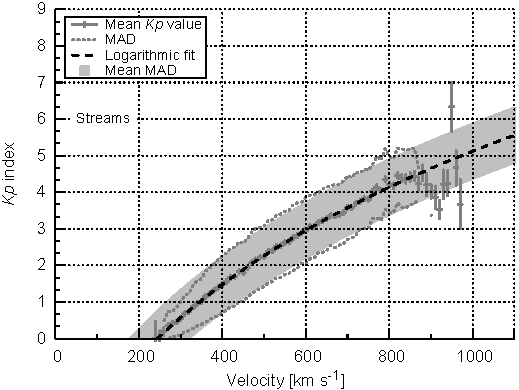
\includegraphics[width=0.6\textwidth]{figures_of_mine/chapter2/Kp_2dhistogram_V_sws23_fit_e.pdf}
	}{
		\caption{Mean \Kp{} values (+) and MAD values (dotted) per velocity interval for the stream part of the data, shifted by 9~hours. The error bars represent the relative data count. The logarithmic fit (dashed) is plotted with a mean MAD band (shaded area). The function (\ref{eq:log_offset_fit_function}) is used for the weighted fit.}
		\label{fig:Kp_2dhistogram_V_sws23_fit_e}
	}
\end{figure}
This leads to the solar-wind stream dependency function
\begin{align}
	\Kp(v) = 5.88 \cdot \ln(v + 299) - 37.0	\,,	\label{eq:kpvsv_sws23_dependency_function}
\end{align}
which can be used to forecast the \Kp{}~index from the estimated stream velocity, e.g., obtained from remote coronal hole analyses.


\section{Discussion and summary}
The following results/relations are obtained from the analyses:
\begin{itemize}
	\item solar activity: \Kp{}-SSN relation with half a \Kp{}~unit as error
	\item seasonal variations: about 1~\Kp{}~unit
	\item solar-wind nowcast: \Kp-\vBz{} relation (average and worst case)
	\item CME forecast: \Kp-velocity relation (average and worst case)
	\item stream forecast: \Kp-velocity relation (average and worst case)
\end{itemize}

CMEs can be faster than the maximal velocities included in the OMNI data. Instrumental effects (specify...) lead to data gaps during these periods. Yet, CME speeds of up to XX~km/s at \SI{1}{\au} were observed in-situ (cite paper ref.). A CME speed of \SI{2000}{\km\per\s} would lead on average to a theoretical \Kp{} of 12.17, however, the \Kp{} scale is capped at 9o. This maximal value is reached already at a velocity of 1489~km/s.\\

Solar-wind streams cannot be faster than 1000~km/s (limited coronal temperatures/never observed (cites?)). That is why streams on average provoke \Kp{} values below 5o.\\

comparison:\\
\Kp-velocity correlation\\
similar to \citet{Elliott2013}; different data time period, resolution and averaging method (3-hour maximum of 1~min data)\\


\section{Applications and outlook}

"scientists develop an advanced prototype space weather warning system to ensure the operation of telecommunication and navigation systems on Earth to the threat of solar storms" AFFECTS\\

Prototype/precursor relations are integrated into applications developed within the Advanced Forecast For Ensuring Communications Through Space (\mbox{AFFECTS}) project which ran from 2011 to 2013. The following services, accessible via the \mbox{AFFECTS} website\footnote{AFFECTS website (existent in 2017-11-19): \url{http://www.affects-fp7.eu/services/}}, contain results from this \Kp{} study (all links existent in 2017-11-19):
\begin{itemize}
	\item DSCOVR real-time solar-wind with \Kp{} plot \url{http://www.affects-fp7.eu/rssfeeds/ace_ap_plot/ace_realtime_ap_plot.png}
	\item DSCOVR real-time solar-wind and \Kp{} forecast plot \url{http://www.affects-fp7.eu/rssfeeds/ace_ap_forecast_plot/ace_realtime_ap_CH_GFT_plot.png}
	\item RSS L1 Kp Alert: \url{http://www.affects-fp7.eu/rssfeeds/rssfeed_kp/rssfeed_kp.xml}
	\item RSS L1 GNSS Alert: \url{http://www.affects-fp7.eu/rssfeeds/rssfeed_gnss/rssfeed_gnss.xml}
	\item RSS L1 Aurora Alert: \url{http://www.affects-fp7.eu/rssfeeds/rssfeed_aurora/rssfeed_aurora.xml}
\end{itemize}

Further applications of resulting \Kp{}-relations:
\begin{itemize}
	\item CME \Kp{} impact (part of UGOE DDC)
	\item iPhone app L1 Alerts (Solar wind latest 2-hour extreme values and derived forecast values): \url{http://www.affects-fp7.eu/app-services/L1-Alerts/dataL1Alerts.txt} \url{https://itunes.apple.com/au/app/affects/id893579846}
	\item Android app L1 Alerts... \url{https://play.google.com/store/apps/details?id=com.afects.forecasts}
	\item has SW-Display Kp forecast??
	\item exclude? Kp forecast calculation: \url{http://www.astro.physik.uni-goettingen.de/~mvenzmer/kp_forecast_calculation/kp_forecast_calculation.php}
\end{itemize}

make real links...\\

reduce list to Kp-related services...\\

outlook:\\
Separate structures such as CIRs and HCSs for their \Kp-impact separately...\\

All provided web links in this work were existent in [date].\\


\section{Acknowledgments}
The research leading to these results has received funding from the European Union's Seventh Framework Programme (FP7/2007-2013) under the grant agreement number 263506 (AFFECTS). The results presented in this paper rely on the \Kp{}~index, calculated and made available by the German Research Centre for Geosciences in Potsdam from data collected at magnetic observatories. We thank the involved national institutes, the INTERMAGNET network and ISGI (isgi.unistra.fr). The authors thank the OMNI PIs/teams for creating and making available the solar-wind in-situ data. The OMNI data are supplied by the NASA Space Science Data Coordinated Archive and the Space Physics Data Facility at NASA's Goddard Space Flight Center. Additional thanks for maintaining and providing the international sunspot number series goes to the World Data Center -- Sunspot Index and Long-term Solar Observations at the Solar Influences Data Analysis Center (SIDC), Royal Observatory of Belgium. The hourly solar wind structure list was kindly provided by Ian~Richardson of the NASA Goddard Space Flight Center and CRESST/University of Maryland via the CEDAR Database at the National Center for Atmospheric Research, which is supported by the National Science Foundation.



